\section{Resultat}

\begin{table}[h!]
	\begin{center}
		\caption{Målinger av de ulike sylindrene.}
		\label{MinLilleTabell}	% Merkelappen vi vil referere til.
		% \vspace{0.5cm}	% Litt ekstra plass for å få det til å se penere ut.
		\begin{tabular}{lrrr} 		% Tre venstrejusterte kolonner (l = left, c = center, r = right).
			\hline 								% Horisontal linje.
		    Sylinder &  masse  & indre diameter & ytre diameter \\ % Merk symboler i kursiv, (men det er fordi de er symboler, ikke fordi de er kolonneoverskrifter!)
			&  (g)    &   (mm)   &  (mm)    \\ % mens enheter ikke er det.
			\hline												
			1   &  442 \(\pm\)0.5 & 	  & 73.5\(\pm\)0.1 \\ % Stor plast solid
			2   &  1097\(\pm\)0.5 & 	  & 44.5\(\pm\)0.1 \\ % Liten metall solid
			3   &  255 \(\pm\)0.5 & 42.4\(\pm\)0.1 & 36.5\(\pm\)0.1 \\ % Liten metall hul
			% Usikkerhet &  \(\pm\)0.5 & \(\pm\) 0.1 & \(\pm\) 0.1 \\
			\hline
		\end{tabular}
	\end{center}
\end{table}


\begin{figure}[p] 
	\begin{center}
        	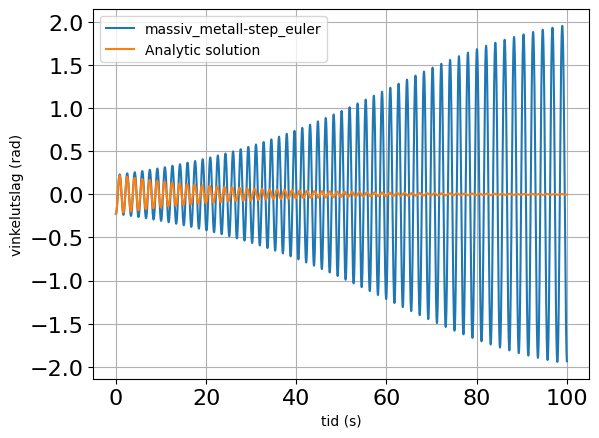
\includegraphics[width=0.45\textwidth]{img/massiv_metall-step_euler.png}
        	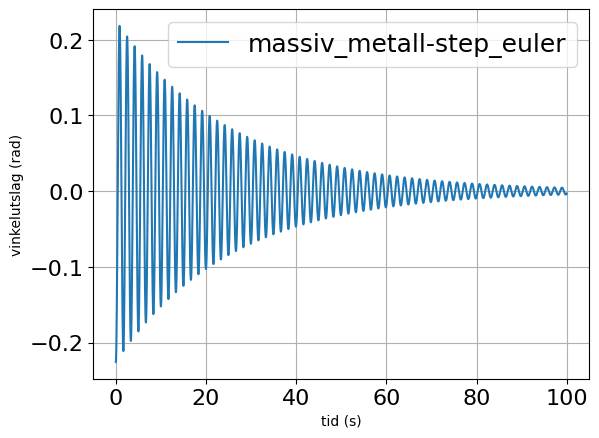
\includegraphics[width=0.45\textwidth]{img/massiv_metall-step_euler-plot.png}
        \end{center}
	\caption{Bruk av Eulers metode. Henholdsvis \(\Delta t = 0.01\) og \(\Delta t = 10^{-6}\).}
	\label{Fig step-Euler} % Som med ligningen, er dette navnet vi refererer til.
\end{figure}

\begin{figure}[p] 
	\begin{center}
		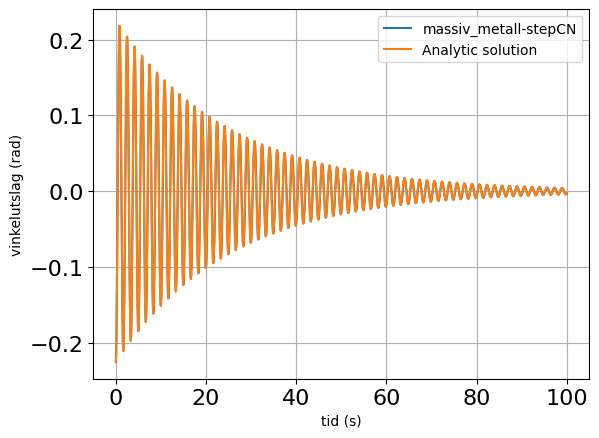
\includegraphics[width=0.45\textwidth]{img/massiv_metall-stepCN.png}
  
 \end{center}
	\caption{CN-metoden og den analytiske løsningen med \(\delta = 0.04\) og \(\beta \text{ og } \phi_R = 0\). Disse sammenfaller fullstendig.}
	\label{Fig CN} % Som med ligningen, er dette navnet vi refererer til.
\end{figure}

\begin{figure}[p] 
	\begin{center}
            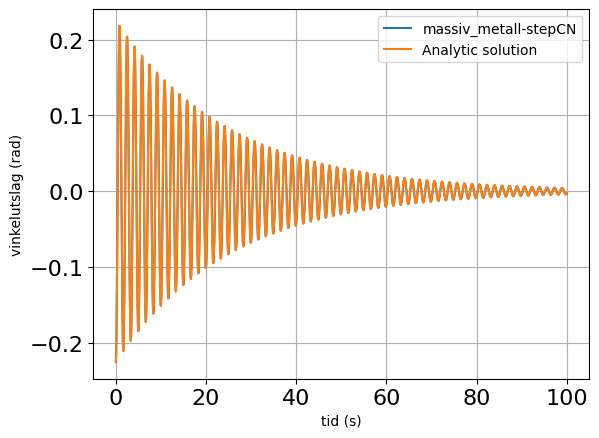
\includegraphics[width=0.45\textwidth]{img/massiv_metall-stepCN.png}
		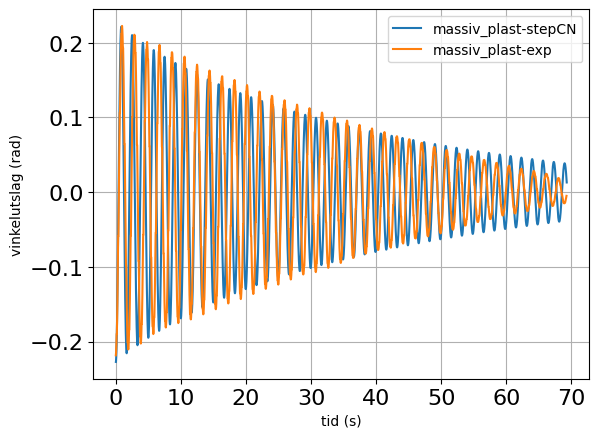
\includegraphics[width=0.45\textwidth]{img/massiv_plast-stepCN copy.png}
 \end{center}
	\caption{Justering av \(\phi_R\), \(\beta\) og \(\delta\) hos helholdsvis massiv metall og massiv plast.}
	\label{Fig tweaking} % Som med ligningen, er dette navnet vi refererer til.
\end{figure}

\begin{figure}[p] 
	\begin{center}
            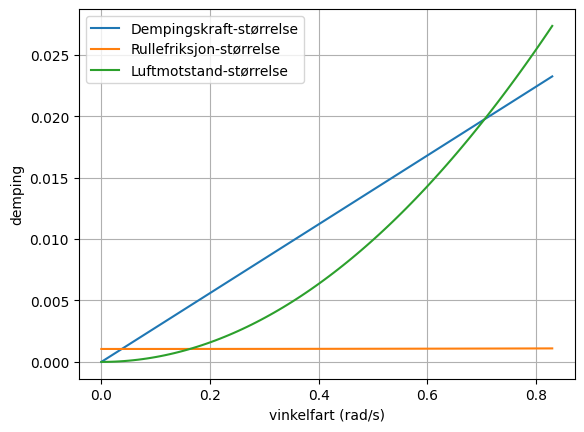
\includegraphics[width=0.45\textwidth]{img/comparison_d_b_r.png}
    \end{center}
	\caption{Sammenligning av påvirkning til \(\phi_R\), \(\beta\) og \(\delta\) som funksjon av \(\dot{\phi}\). Ser på tidspunkt med maksimal rullemotstand når \(\phi = 0\). Det er bare rullefriksjonsleddet som avhenger av \(\phi\) (se \eqref{ODE}).}
	\label{Fig comparison} % Som med ligningen, er dette navnet vi refererer til.
\end{figure}

Figur \ref{Fig step-Euler} viser implementering av Eulers metode på måle\-serien til Sylinder 1. Her er det valgt \(\Delta t = 0.01\) og \(\Delta t = 10^{-6}\). 
Crank-Nicholson-metoden gir fullstendig sammenfallende løsning som den analytiske løsningen av \eqref{ODE}. Se figur \ref{Fig CN}.

Eksperimentering av ulike verdier for \(\phi_R\), \(\delta\) og \(\beta\) gir figur \ref{Fig tweaking} som beste resultat. Her er \(\delta = 0.014\), \(\phi_R = 0.0002\) og \(\beta = 0.080\) hos massiv metall og \(\delta = 0.009\), \(\phi_R = 0.0006\) og \(\beta = 0.090\) hos massiv plast.
\par
Brukte videre \eqref{ODE} for å plotte hvordan de ulike dempeleddene i differensialligningen varierer med \(\dot{\phi}\) (se figur \ref{Fig comparison}).
